
% 放物線補間 (SPI) のアニメーション
\begin{frame}{放物線補間の収束プロセス}
  \begin{columns}
    \begin{column}{0.4\textwidth}
      \begin{itemize}
        \item \textcolor{blue}{\textbf{青丸}}: 補間に使用する3点
        \item \textcolor{green}{\textbf{緑破線}}: 3点を通る近似放物線
        \item \textcolor{red}{\textbf{赤丸}}: 放物線の頂点 
      \end{itemize}
      \vspace{1em}
      \small
      頂点付近では極めて高速に収束するが、初期値が悪いと放物線が反転して遠くへ飛んだり、更新が停滞したりするリスクがある。
    \end{column}
    \begin{column}{0.6\textwidth}
      \centering
      \only<1>{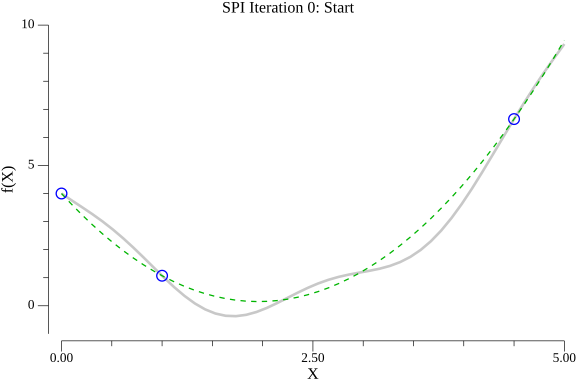
\includegraphics[width=\textwidth]{material/spi/output/spi_00.png}}
      \only<2>{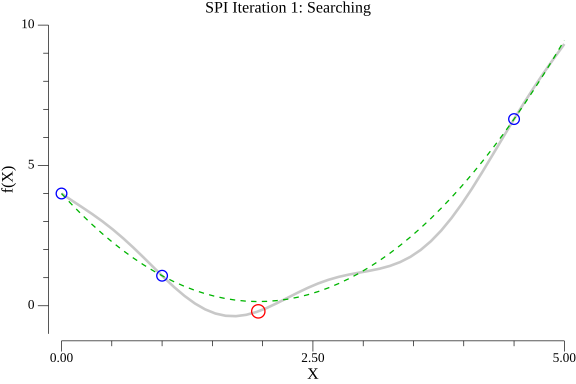
\includegraphics[width=\textwidth]{material/spi/output/spi_01.png}}
      \only<3>{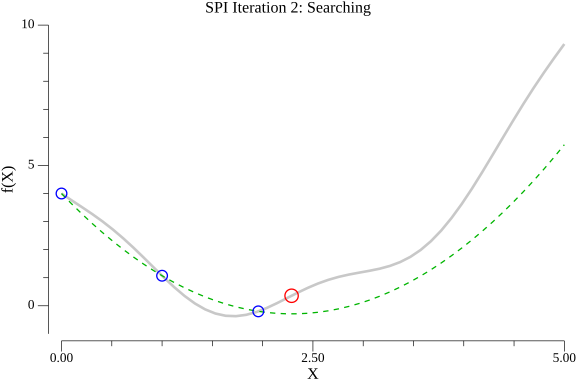
\includegraphics[width=\textwidth]{material/spi/output/spi_02.png}}
      \only<4>{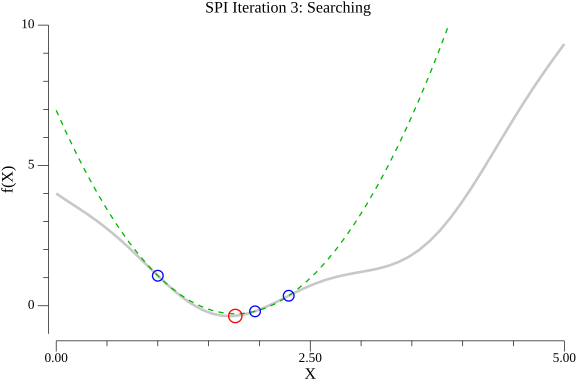
\includegraphics[width=\textwidth]{material/spi/output/spi_03.png}}
      \only<5>{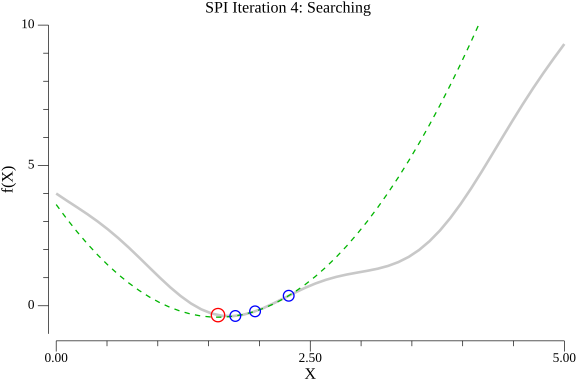
\includegraphics[width=\textwidth]{material/spi/output/spi_04.png}}
      \only<6>{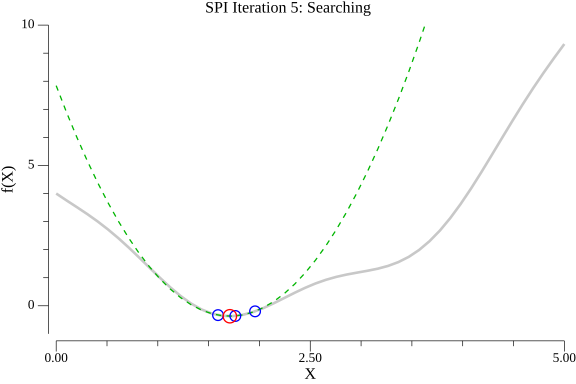
\includegraphics[width=\textwidth]{material/spi/output/spi_05.png}}
      \only<7>{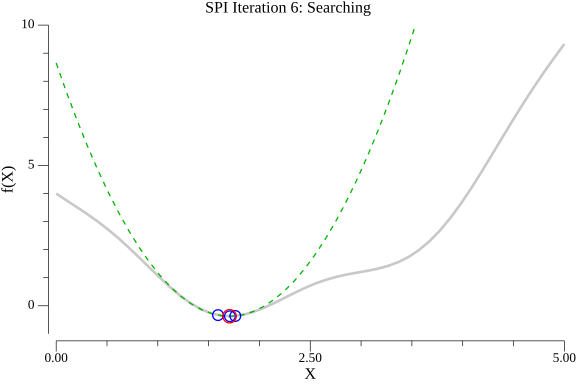
\includegraphics[width=\textwidth]{material/spi/output/spi_06.png}}
      \only<8>{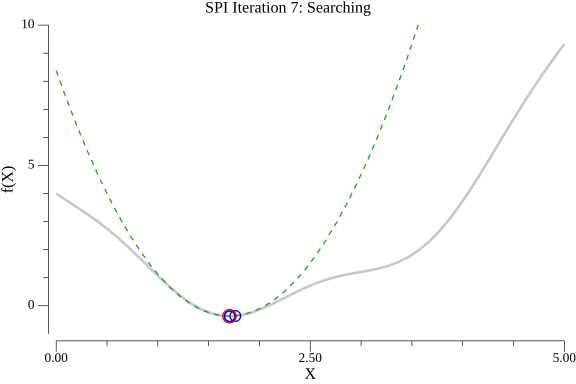
\includegraphics[width=\textwidth]{material/spi/output/spi_07.png}}
      \only<9>{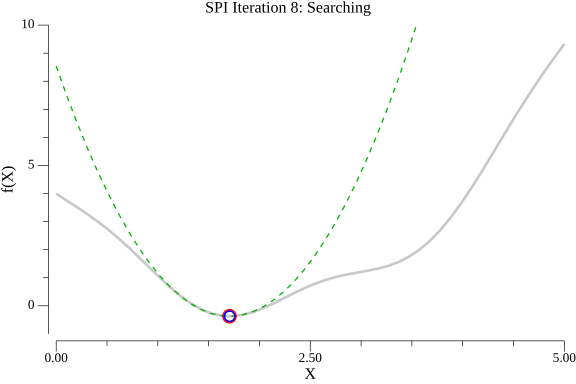
\includegraphics[width=\textwidth]{material/spi/output/spi_08.png}}
      \only<10>{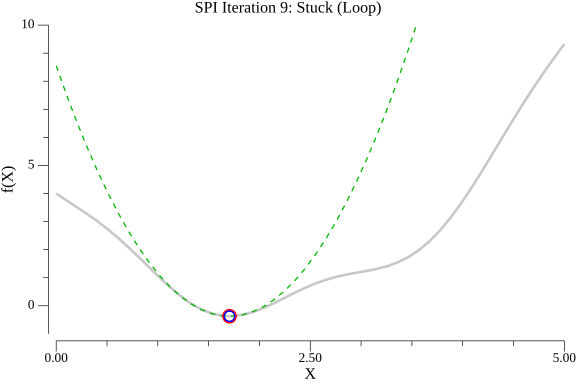
\includegraphics[width=\textwidth]{material/spi/output/spi_09.png}}
    \end{column}
  \end{columns}
\end{frame}
